\documentclass[lettersize,journal]{IEEEtran}
\usepackage[T1]{fontenc}
\usepackage{amsmath,amssymb}
\usepackage{array}
\usepackage{booktabs}
\usepackage{graphicx}
\usepackage{cite}
\usepackage{url}
\usepackage{xcolor}
\usepackage{microtype}
\usepackage{hyperref}
\usepackage[capitalize,noabbrev]{cleveref}
\hypersetup{hidelinks}
\graphicspath{{figures/}}
\hyphenation{hetero-geneous accel-erator coher-ency}

\begin{document}

\title{AIRTOS: Evidence-Constrained Admission, Resource Governance, and Recovery for Heterogeneous Edge AI}

\author{Anonymous Authors}

\maketitle

\begin{abstract}
Heterogeneous edge-AI inference spans CPU, vector, accelerator, and DMA
resources while sharing bounded memory and non-coherent buffers. A plan that
is valid at compile time may therefore be ineligible for the current input,
device state, memory state, admitted workload, or recovery budget. This
article presents AIRTOS, an evidence-constrained runtime governance layer that
treats the execution plan as a first-class operating-system object. AIRTOS
combines package and evidence validation, provider and input checks, arena
allocation, coherency requirements, all-job schedule simulation, and recovery
policy in one admission decision. It atomically publishes the job and its
memory lease, dispatches dependency-ready segments through per-resource
earliest-deadline-first queues, executes plan-declared ownership transitions,
and identifies every completion by device epoch and dispatch cookie. Fallback
re-enters the same admission path rather than bypassing the original
constraints. We implement AIRTOS on RT-Smart and evaluate a frozen
49,085,520-byte corpus on x86\_64, RV64 QEMU user mode, five QEMU system models,
and a CanMV-K230-LP4 V3.0 platform. In each of two non-HIL runs, every system
model replayed 7,950 loader, 24,548 scheduling, and one million coherency cases
without a decision mismatch or state-machine failure. On K230, no registered
safety failure was observed across 24,548 simulator-oracle comparisons,
400,000 concurrent admissions, one million lease attempts, one million
physical DMA transfers, 700,000 stale-event injections, and 7,500 recovery and
fallback episodes. All 800 omitted-cache-operation controls were detected,
and a 24-minute run completed 6,685,424 DMA lifecycle iterations without a
data, device-call, or lifecycle failure. Board measurements also exceeded the
registered CPU and RVV execution bounds, causing AIRTOS to reject the timing
contract and require requalification. These results show that AIRTOS can
govern plan eligibility, execution, and failure recovery with explicit and
auditable runtime conditions.
\end{abstract}

\begin{IEEEkeywords}
Edge AI, heterogeneous computing, admission control, real-time systems,
runtime assurance, DMA coherency, fault recovery.
\end{IEEEkeywords}

\section{Introduction}
\IEEEPARstart{E}{dge} inference increasingly crosses a qualification boundary
that conventional deployment interfaces leave implicit. A compiler emits an
execution plan under a target and timing model, whereas the operating system
must execute it under live provider, memory, cache, and workload conditions.
The inference itself may be a directed acyclic graph (DAG) of CPU, vector,
accelerator, and DMA segments rather than one schedulable thread. Consequently,
structural validity and numerical correctness do not by themselves establish
that a plan is eligible to run at a particular instant.

Consider an industrial vision controller that serves defect inspection,
personnel recognition, and thermal-anomaly detection concurrently. The jobs
share an accelerator and bounded on-chip memory, but they use different
sequences of preprocessing, transfer, neural or vector computation, and
postprocessing. A new defect-detection plan may be correct in isolation while
its input lies outside the qualified domain, its provider is recovering, its
arena is unavailable, or its deadline interferes with an accepted thermal
job. After a timeout, a pre-reset completion may also arrive during a new
command, while a slower fallback may invalidate earlier deadline commitments.
The operating system must resolve these conditions over the complete job
lifecycle.

The conventional path compresses these decisions into one inference call:
compile the model, invoke the runtime, and wait for the device. AIRTOS instead
validates the plan and its evidence, checks the invocation and provider,
probes memory, recomputes all outstanding deadlines, and atomically publishes
the job and lease. Execution follows explicit ownership and completion rules;
timeout, cancellation, reset, quarantine, and fallback remain inside the same
protocol. The admission question therefore becomes whether the plan can run
now while preserving the resource, data, and timing commitments already made
by the system.

The toolchain separates this responsibility into three stages. Compilation
constructs a target-specific execution plan, and evidence production records
the input domain and conditions under which the plan was qualified. AIRTOS
then governs the transition from that qualified plan to physical execution.
It admits the plan only when its evidence, invocation, providers, memory,
deadline commitments, coherency actions, and recovery policy agree with the
current system state. This consumer-side boundary complements compilation and
evidence production with a runtime decision that neither preceding stage can
make in advance.

Real-time scheduling theory makes the assumptions behind timing guarantees
explicit. Classical EDF and sporadic-task feasibility analysis depend on
bounded execution and defined arrival models
\cite{liu1973scheduling,baruah1990preemptively}; execution-time assurance work
further shows that the strength of a timing claim is inseparable from the
bounds supplied to the scheduler \cite{vestal2007preemptive}. Heterogeneous
task runtimes and schedulers already express DAG dependencies, locality, and
resource types \cite{topcuoglu2002performanceeffective,augonnet2011starpu,
bauer2012legion,rossbach2011ptask,lin2022typeaware}. Accelerator-sharing
systems likewise address preemption, spatial partitioning, memory pressure,
and multi-model quality of service
\cite{choi2020prema,ghodrati2020planaria,kim2023moca,kim2023dream}. These
mechanisms provide the scheduling and resource foundations used by AIRTOS.
Their normal entry point, however, is a workload whose execution model has
already been accepted.

AIRTOS closes this gap with one joint predicate over parsing, binding,
applicability, evidence, providers, memory, coherency, timing, and recovery.
Admission probes an arena lease and evaluates a conservative multi-resource
schedule against both existing and candidate jobs. It publishes memory and
job state only when their generations remain unchanged. Dependency-ready
segments then enter stable per-resource EDF queues, plan-declared actions
transfer buffer ownership, and epoch-cookie pairs associate completion events
with the active device command. A bounded recovery policy either restores or
quarantines a provider, and every fallback passes through the complete gate.

The design follows the separation principle used in runtime assurance: a
producer proposes an action, while a consumer-side mechanism decides whether
that action is admissible in the present state
\cite{seto1998simplex,hobbs2023runtime}. Trace records are similarly
scoped. They select a subsequent compiler experiment without elevating
evidence or installing a plan directly; every candidate returns through
verification and admission. Runtime observation can therefore guide
optimization while remaining separate from qualification
\cite{leucker2009brief}.

We evaluate AIRTOS through four claim-oriented cores, two complete non-HIL
runs, a five-model QEMU system matrix, and a physical HIL run. The frozen
corpus is replayed across x86\_64, RV64 user mode, RT-Thread/RV64, and
Cortex-M3/M4/M7 system models before the physical K230 data path is exercised.
The experiments cover qualification decisions, concurrent memory--schedule
transactions, an independent scheduling oracle, arena leases, coherency
state-machine decisions, physical DMA controls, stale-event and recovery
transitions, fallback gates, and trace classification. The timing audit also
tests whether measured execution remains inside the plan contract. CPU and RVV
maxima exceeded their registered bounds, and the admission evidence was
accordingly marked for requalification.

This work makes four contributions:
\begin{enumerate}
  \item an evidence-constrained admission predicate that combines plan
  qualification with live resource, memory, coherency, timing, and recovery
  state;
  \item an optimistic atomic lease-and-schedule transaction that prevents
  half-admitted jobs under concurrent submissions;
  \item dependency-aware resource governance with explicit ownership
  transitions and epoch-scoped completion and recovery semantics; and
  \item a claim-oriented evaluation that combines independent decision
  oracles, physical coherency controls, recovery endpoints, and timing-contract
  auditing.
\end{enumerate}
The novelty lies in composing these mechanisms under one consumer-checkable
plan lifecycle, from qualification and publication through completion,
recovery, fallback, and feedback.

The remainder of this paper follows the lifecycle of a governed plan.
Section~II positions the qualification boundary against scheduling,
heterogeneous runtimes, runtime assurance, and DMA ownership. Section~III
defines jobs, runtime state, admission, and the conditional properties that
connect the model to execution. Section~IV then presents the end-to-end AIRTOS
procedure and explains its principal design choices. Sections~V and~VI describe
the implementation and claim-oriented experimental method, respectively.
Section~VII evaluates admission, memory and coherency, recovery, feedback, and
timing applicability, after which Sections~VIII and~IX discuss the resulting
operational contract and conclude.

\section{Background and Related Work}
\subsection{Real-Time and Heterogeneous DAG Scheduling}
Liu and Layland establish the classical uniprocessor foundation for EDF under
periodic-task assumptions \cite{liu1973scheduling}, while processor-demand
analysis extends feasibility reasoning to sporadic workloads
\cite{baruah1990preemptively}. Vestal makes execution-time assurance an
explicit scheduling dimension \cite{vestal2007preemptive}. AIRTOS retains this
discipline: its deadline statement is conditional on registered segment costs,
non-preemptive blocking, modeled arrivals, coherency charges, and recovery
charges. Its simulator rechecks all admitted deadlines after candidate
insertion instead of treating EDF priority as a timing proof.

HEFT schedules precedence-constrained tasks across heterogeneous processors
using rank-based list scheduling \cite{topcuoglu2002performanceeffective}.
StarPU combines task scheduling with heterogeneous data management
\cite{augonnet2011starpu}; Legion expresses independence and locality through
logical regions \cite{bauer2012legion}; and PTask makes accelerator work and
dataflow visible to the operating system \cite{rossbach2011ptask}. Type-aware
federated scheduling gives real-time semantics to typed heterogeneous DAGs
\cite{lin2022typeaware}. AIRTOS does not present DAG queues or per-resource EDF
as new algorithms. It places these mechanisms downstream of an evidence and
applicability gate and couples their result to a generation-checked memory
transaction and recovery state.

\subsection{Accelerator Runtimes and Multi-Tenant AI}
Accelerator sharing spans different hardware assumptions. PREMA exploits
preemptible NPU execution \cite{choi2020prema}, whereas Planaria partitions an
accelerator spatially among tenants \cite{ghodrati2020planaria}. MoCA adapts
execution around multi-tenant memory behavior \cite{kim2023moca}, and DREAM
targets dynamic real-time multi-model edge workloads \cite{kim2023dream}.
Salus exposes fine-grained GPU sharing primitives and distinguishes persistent
from transient memory \cite{yu2019salus}; Clockwork pursues predictable DNN
serving through controlled execution and explicit timing information
\cite{gujarati2020serving}. These systems establish that scheduling, memory,
and latency must be governed jointly. Their admitted unit, however, is
generally a model or execution request rather than a plan carrying separately
checkable domain and evidence obligations.

Embedded inference systems demonstrate how tightly runtime design is coupled
to constrained memory and platform support. TensorFlow Lite Micro provides an
embedded inference runtime for small devices \cite{david2021tensorflow}, and
MLPerf Tiny establishes reproducible measurement practices for such platforms
\cite{banbury2021mlperf}. AIRTOS focuses on the qualification layer: whether a
particular evidence-carrying plan may enter the live runtime and how its
memory, timing, ownership, and recovery obligations remain governed.

\subsection{Runtime Assurance, Coherency, and Recovery}
Simplex separates a high-performance controller from a trusted baseline and
decision module \cite{seto1998simplex}; modern runtime-assurance work
generalizes that structure as a safety filter around complex components
\cite{hobbs2023runtime}. Runtime verification checks execution events against
specified properties \cite{leucker2009brief}. AIRTOS applies the separation at
the compiler--runtime boundary: a producer supplies a plan and evidence, while
the runtime checks current eligibility. Its trace can only propose an
experiment, preventing an execution from certifying its replacement.

DMA specifications already define fences and ownership transitions for
asynchronous devices \cite{documentation2026buffer,documentation2026dma}.
AIRTOS does not redefine these primitives. Instead, the plan names the buffer
range and required clean, barrier, and invalidate actions; the runtime confines
the range to the active lease and invokes provider hooks at the ownership
boundary. Completion attribution adds an orthogonal device-generation rule:
an event is accepted only when resource, epoch, active command, and cookie
agree. The evaluation uses an independent scheduling oracle rather than
deriving expected answers from the runtime under test, following the principle
that oracle construction is part of the validity argument \cite{barr2015oracle}.

\subsection{The Qualification Gap}
Prior systems provide the mechanisms from which AIRTOS is built, but they
place their acceptance boundaries at different points. A scheduler assumes a
task model and asks whether a priority or placement decision is feasible. A
heterogeneous runtime assumes that submitted kernels and buffer descriptions
are valid and decides where and when to execute them. Runtime assurance
filters a proposed action against a monitored state, while DMA interfaces
define how software transfers buffer ownership. The unresolved boundary lies
before all four: deciding whether the submitted plan, its evidence, its input,
and the current machine state jointly constitute a valid scheduling object.

A plan-level decision cannot be replaced by a sequence of independent API
checks. A lease allocated before schedule simulation may remain stranded when
the timing test fails. Conversely, a schedule accepted before allocation can
become unrealizable under memory pressure. A candidate-only deadline test can
approve the new job even when it delays an older commitment, and a fallback
selected only because its provider is healthy can still carry stale evidence
or an infeasible execution bound. AIRTOS makes these dependencies explicit by
placing one consumer-side predicate and one atomic publication point around
the plan lifecycle.

This placement also clarifies the trust split. The compiler is authoritative
for the plan structure it emits, and the evidence stage is authoritative for
the conditions under which the plan was qualified. The runtime is
authoritative for changing facts: invocation values, provider health, active
leases, queued and running work, recovery state, and the current trust policy.
None of these authorities substitutes for another. The composition preserves
the specialized analyses of the producer while giving the operating system a
small, checkable basis for deciding whether their result can enter physical
execution.

\section{System Model and Problem Formulation}
\subsection{Operating and Failure Model}
AIRTOS runs inside a heterogeneous edge system containing CPU, vector, NPU,
and DMA providers connected through a bounded arena and potentially
non-coherent cached memory. Providers may execute concurrently, while one
active command on a provider is non-preemptive. The runtime receives a
compiler package, an invocation, an absolute deadline, and a minimum evidence
policy. It also observes the current provider registry, lease map, admitted
jobs, reservations, device epochs, and recovery budgets. These observations
form the state against which eligibility is decided.

The failure model includes malformed or mismatched package fields, input
values outside the declared domain, insufficient evidence coverage, provider
unavailability, arena exhaustion, infeasible deadline interference, missing
coherency actions, timeouts, duplicate or delayed completions, and failed
recovery attempts. Concurrency can change provider, lease, or schedule state
while a candidate is being checked. AIRTOS therefore treats check--commit
races as part of the correctness problem. Package parsing, evidence policy,
provider hooks, cache operations, and the monotonic clock belong to the trusted
computing base for their stated contracts; the compiler plan itself remains
untrusted until every consumer-side check succeeds.

The system also distinguishes three kinds of time. Registered segment cost is
the conservative quantity used by admission. Hardware completion is the event
reported by a provider. Logical completion is the point at which AIRTOS makes
successors and resources visible to its scheduling model. Keeping these times
separate prevents a favorable measurement or an early device interrupt from
silently changing the model under which existing jobs were accepted.

\subsection{Jobs, Plans, and Runtime State}
An admitted job is
\begin{equation}
J_i=(id_i,P_i,r_i,d_i,\kappa_i,\chi_i),
\end{equation}
where $P_i$ is a compiler-produced plan, $r_i$ is release time, $d_i$ is an
absolute deadline, $\kappa_i$ is the minimum evidence policy, and $\chi_i$ is
a recovery policy. A plan contains a segment DAG $G_i=(V_i,E_i)$. Each segment
is
\begin{equation}
s=(id,res,C,Pred,off,size,flags),
\end{equation}
where $res\in\{CPU,RVV,NPU,DMA\}$, $C$ is a registered execution bound,
$Pred$ is the predecessor set, $off$ and $size$ identify a lease-relative
buffer range, and $flags$ declare ownership actions. A segment becomes ready
only after release and completion of every predecessor:
\begin{equation}
Ready(s,t)\Leftrightarrow t\ge r_i\land
\forall u\in Pred(s),\ state(u)=done.
\end{equation}

The runtime state is
\begin{equation}
R_t=(\{Q_r\},\{A_r\},\mathcal L,\mathcal C,
\{epoch_r\},\{cookie_r\},D_t,Z_t),
\end{equation}
where $Q_r$ and $A_r$ are the ready queue and active segment for resource $r$,
$\mathcal L$ is the active lease set, $\mathcal C$ is buffer ownership state,
$D_t$ records provider health and recovery, and $Z_t$ is the attributable
trace. Each queue is ordered by the owning job's absolute deadline with stable
FIFO tie-breaking. Running device segments are non-preemptive.

\subsection{Evidence-Constrained Admission}
AIRTOS admits a candidate only when nine conditions hold jointly:
\begin{align}
Admit(J_i,R_t)\Leftrightarrow{}&Parse\land Bind\land Domain\land Evidence
\nonumber\\
&\land Provider\land Memory\land Coherence\nonumber\\
&\land Sched\land Recoverable.
\label{eq:admit}
\end{align}
$Parse$ covers safe package decoding. $Bind$ links package, plan, model,
target, runtime ABI, provider ABI, and fallback identities. $Domain$ covers
shape, dtype, layout, and byte ranges. $Evidence$ requires every selected
obligation to have the expected scope, artifact, verifier identity, resource,
and verified status. $Provider$ requires registered and healthy resources.
$Memory$ requires a non-overlapping lease that contains all declared ranges.
$Coherence$ requires supported ownership actions. $Sched$ requires all old and
new jobs to meet their deadlines in simulation. $Recoverable$ requires valid
budgets and a resource that is neither pending recovery nor quarantined.

The scheduling term is evaluated by $SimEDF^+$, a discrete-event simulation
with per-resource non-preemptive EDF, DAG releases, active residuals,
coherency and recovery charges, and reservation demand. For a running segment
started at $t_s$, the charged residual is
\begin{equation}
C_s^{rem}=\max(0,C_s-(t-t_s))+O_s^{coh}+O_s^{rec}.
\end{equation}
The candidate passes only if
\begin{equation}
\forall J_j\in\mathcal J_{admitted}\cup\{J_i\},\quad
\widehat F_j\le d_j,
\label{eq:alljobs}
\end{equation}
and reservation demand at each checked horizon does not exceed supply. The
all-job test is necessary because an earlier-deadline candidate can finish on
time while delaying a previous commitment beyond its deadline.

\subsection{Safety Properties and Conditional Timing}
\textit{Lease isolation:} if leases are pairwise disjoint, the loader confines
segment ranges to the plan arena, and providers access only declared ranges,
then segments from different sessions address disjoint intervals. This property
concerns inter-session isolation; within-session alias validity remains part of
the compiler plan.

\textit{DAG order:} if a segment enters a resource queue only after all
predecessors complete and only queued segments dispatch, every dispatch
sequence is a topological extension of the plan DAG. EDF orders ready segments
but does not bypass dependencies.

\textit{Epoch isolation:} a completion event carries $(r,e,c,status)$. It is
accepted only if
\begin{equation}
Accept(irq,R_t)\Leftrightarrow e=epoch_r\land c=cookie_r
\land A_r\ne\varnothing.
\label{eq:accept}
\end{equation}
A reset advances the epoch, so an event from an earlier generation cannot
mutate a new command. Valid completion clears active association, rejecting a
same-epoch duplicate; cookie wrap advances the epoch before reuse.

\textit{Conditional data consistency:} for a non-coherent buffer, AIRTOS
models
\begin{equation}
\begin{aligned}
CPU_{dirty}&\xrightarrow{clean+barrier}Device,\\
Device&\xrightarrow{complete+invalidate}CPU_{valid}.
\end{aligned}
\end{equation}
If the plan declares the correct range and actions, provider hooks implement
them, and the device obeys completion semantics, device reads observe submitted
CPU data and later CPU reads observe device output.

\textit{Conditional deadline safety:} let a segment dispatch at $a_s$,
complete in hardware at $h_s$, and have registered budget $C_s$. AIRTOS exposes
logical completion at
\begin{equation}
\ell_s=\max(h_s,a_s+C_s).
\label{eq:logical}
\end{equation}
Holding early completion to the modeled boundary keeps successor releases and
non-preemptive occupancy aligned with $SimEDF^+$. If actual execution and
charged overhead do not exceed registered bounds, arrivals and faults remain
inside reservation, all jobs pass atomic admission, and runtime tie-breaking
matches simulation, the schedules coincide by induction over events. A passing
all-job check then preserves the deadline invariant. An execution exceeding its
registered bound leaves this timing domain and requires requalification.

\textit{Atomic publication:} consider a successful submission at the locked
publication step. The lease generation and schedule generation have just been
revalidated, the arena commit has succeeded, and no subsequent operation before
job publication can fail. Hence a visible job owns a committed lease, while a
rejected or retried submission publishes neither. The generation checks extend
this argument to concurrent admissions by invalidating every stale probe or
schedule snapshot before publication.

\textit{Bounded recovery closure:} if cancellation, reset, and reinitialization
polls respect their declared budgets and at most $K_r$ reset attempts are
permitted, a recovering resource reaches either healthy or quarantined state in
finite model time. Retaining the failed job's lease until closure prevents the
same range from being reassigned while an old device command can still exist.

\subsection{Governance Objectives}
The preceding properties induce four runtime objectives. First,
\emph{qualification integrity} requires that a published job retain the exact
package, target, model, ABI, input-domain, and evidence bindings evaluated at
admission. Second, \emph{resource integrity} requires a published job to own a
non-overlapping lease and to dispatch only dependency-ready segments to healthy
providers. Third, \emph{temporal non-interference} requires candidate insertion
to preserve every earlier deadline commitment under the registered cost and
arrival model. Fourth, \emph{failure closure} requires every accepted command
to reach completion, bounded recovery, or quarantine without permitting an
old completion or an unchecked fallback to mutate the new state.

These objectives are compositional. Lease isolation alone says nothing about
deadline feasibility; schedule feasibility says nothing about cache ownership;
and correct cancellation says nothing about a completion that arrives after
reset. A successful lifecycle therefore requires all objectives at their
respective transition points. Admission establishes the initial conjunction,
dispatch preserves dependency and ownership state, completion preserves
attribution, and recovery restores a state from which admission can be
evaluated again.

\section{AIRTOS Design}
\subsection{Evidence Flow and Governance}
AIRTOS consumes an AEG v2 package containing plan and evidence identities,
policy and target bindings, input domain, segment DAG, execution costs, arena
size, ownership actions, reservation parameters, fallback identity, and
recovery budget. Session creation validates structure before accessing payload
objects, compares the package against a consumer-side trust bundle, and checks
each evidence obligation independently. Submission adds invocation-specific
checks and current provider, memory, schedule, and recovery state.

Table~\ref{tab:contract} organizes the package as five runtime contract
dimensions. The first two rows establish plan identity and input
applicability. The resource and timing rows connect that qualified plan to the
current provider, lease map, ownership state, and all-job schedule. The final
row keeps recovery and feedback under the same contract, so neither path can
introduce an alternate route to execution.

\begin{table}[t]
\caption{Plan Contract and Consumer-Side Enforcement}
\label{tab:contract}
\centering
\footnotesize
\begin{tabular}{@{}p{0.31\columnwidth}p{0.60\columnwidth}@{}}
\toprule
Contract dimension & Runtime enforcement \\
\midrule
Package and identities & Bounds-safe load; plan/model/target/ABI and fallback binding \\
Input and evidence & Shape/dtype/layout/bytes; obligation scope, artifact, verifier, resource, status \\
Resources and memory & Provider health; lease range, generation, and segment bounds \\
Timing and ownership & All-job $SimEDF^+$; declared clean/barrier/invalidate actions \\
Recovery and feedback & Timeout/attempt budget, quarantine, fallback re-admission, non-promoting trace \\
\bottomrule
\end{tabular}
\end{table}

\begin{figure*}[t]
  \centering
  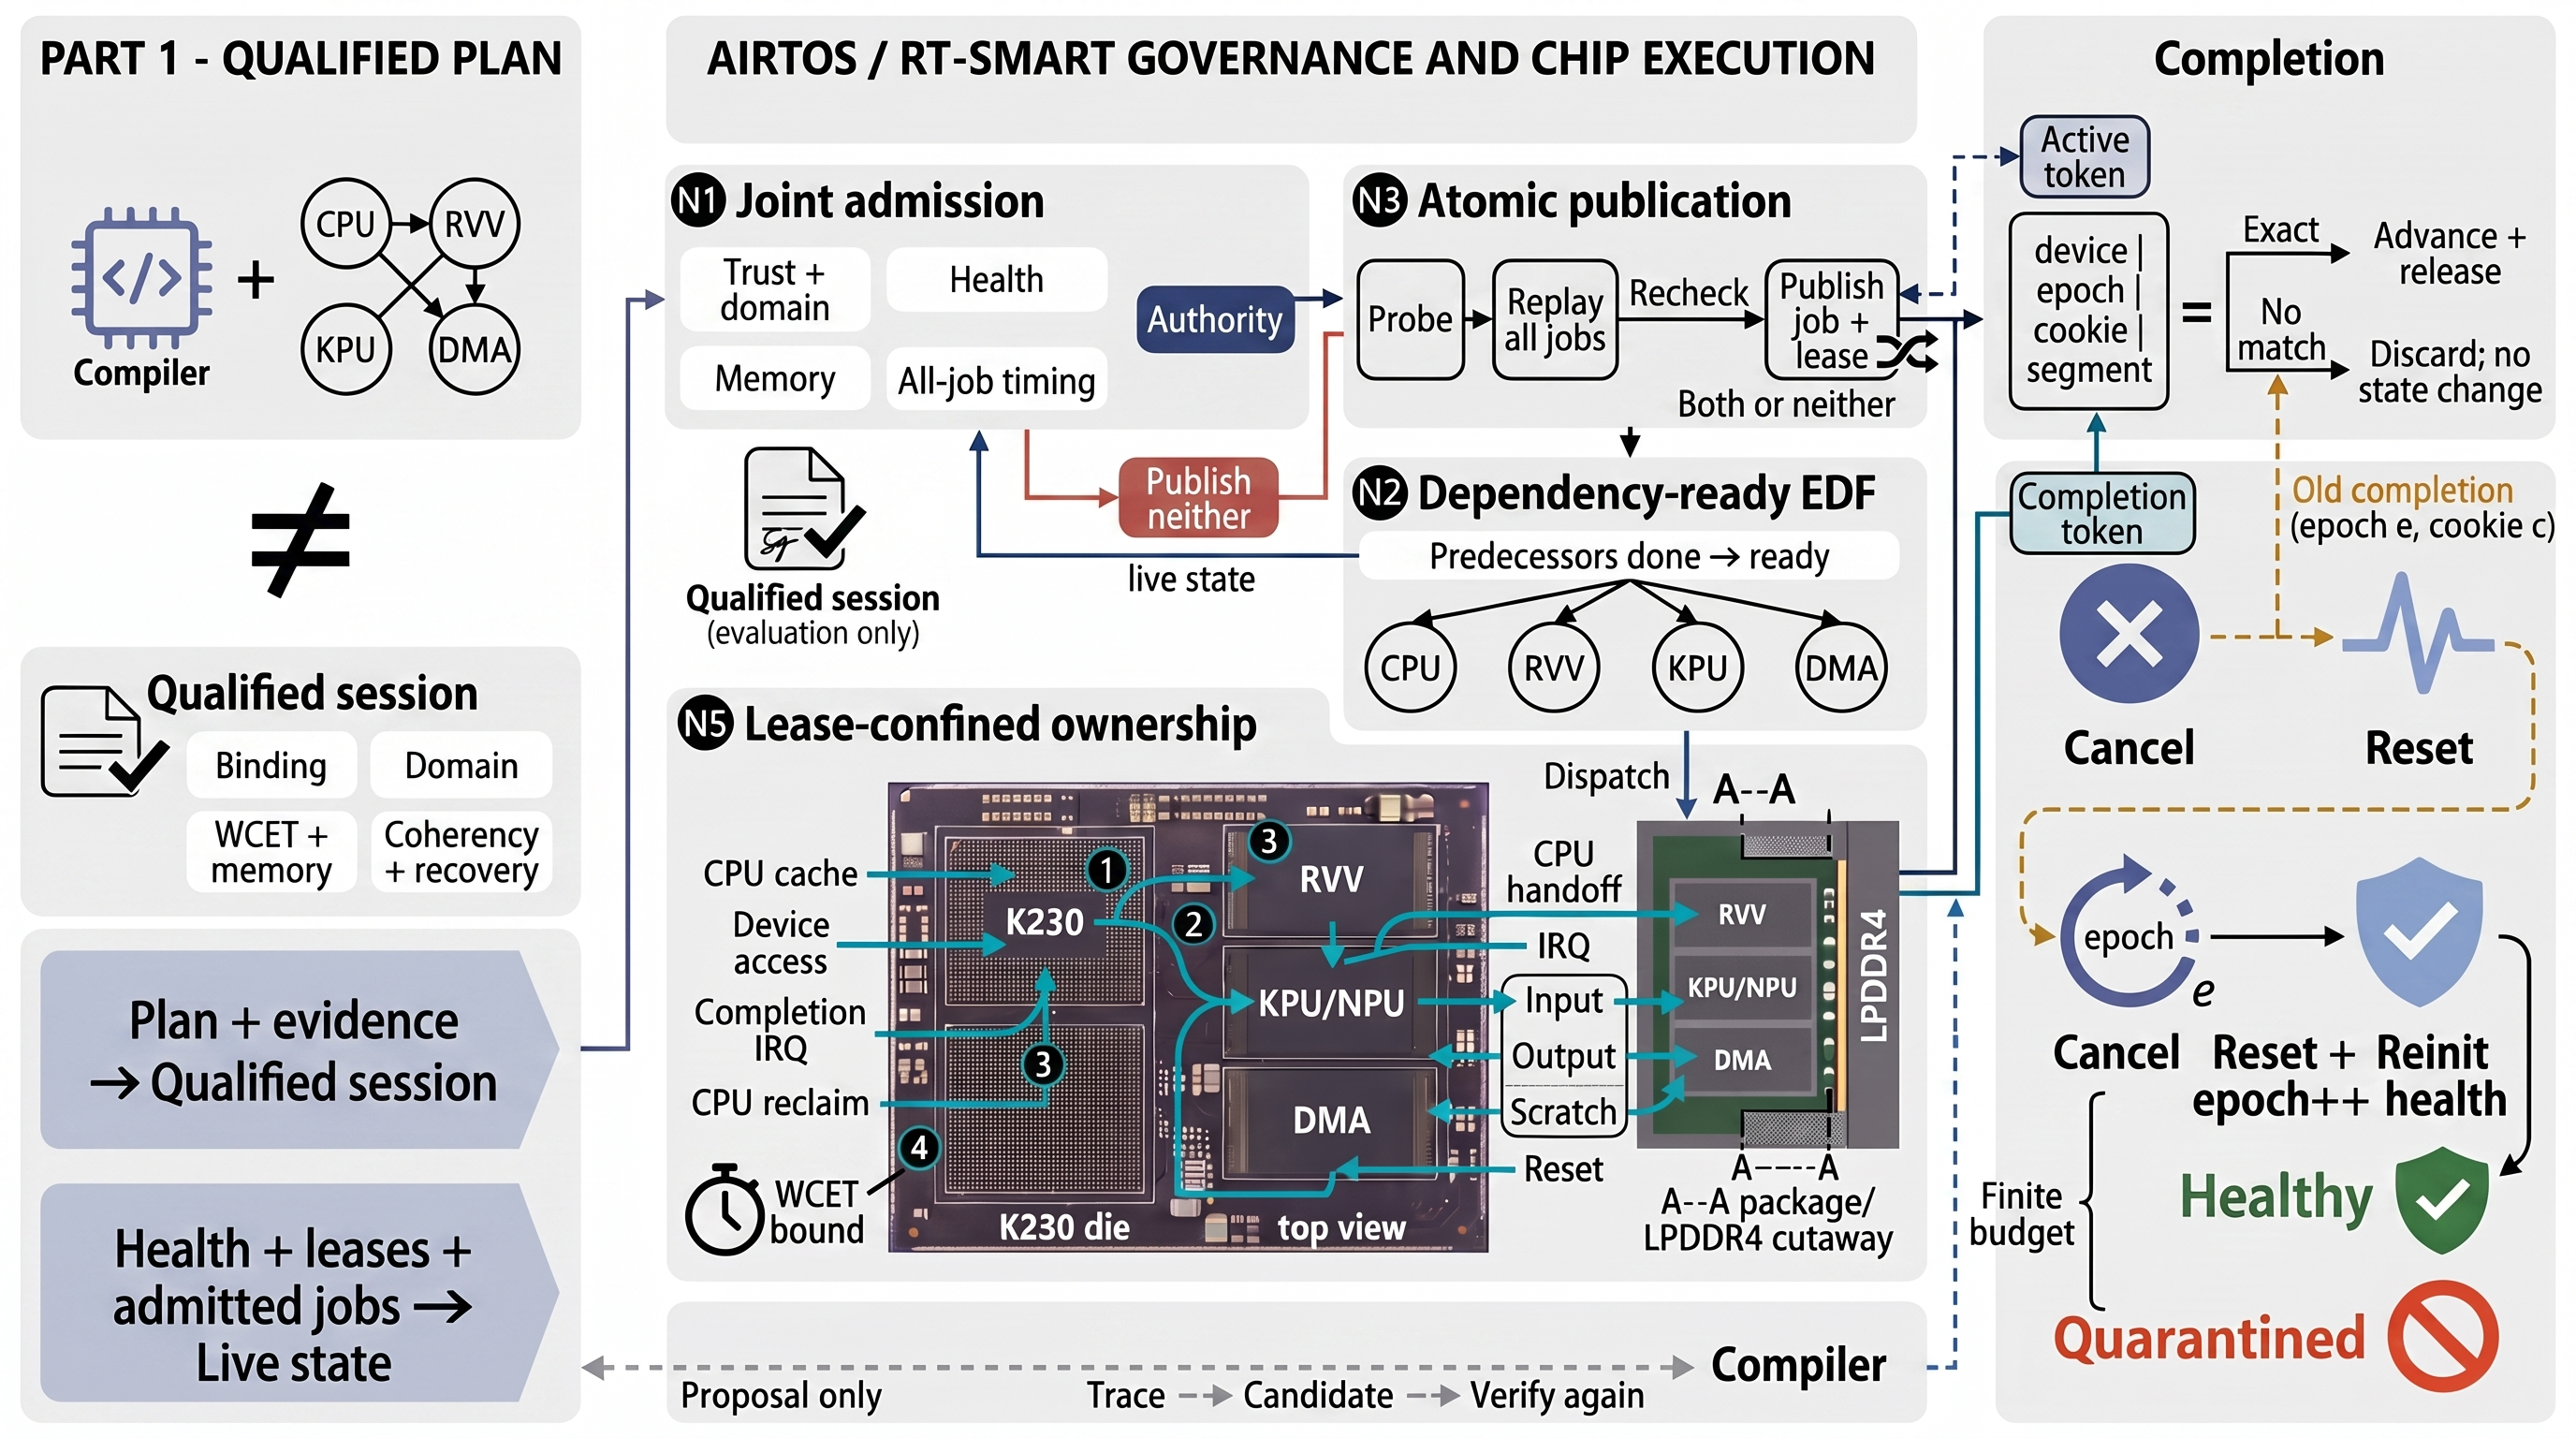
\includegraphics[width=\textwidth]{fig_airtos_main.png}
  \caption{AIRTOS as an execution-authority lifecycle. N1 and N3 transform a
  qualified session plus live state into one atomic job--lease publication;
  N2 and N5 bind the resulting dispatch token to heterogeneous execution and
  physical ownership; N4 either consumes an exact-match completion or revokes
  authority through bounded recovery, while N6 can only propose a reverified
  compiler experiment.}
  \label{fig:architecture}
\end{figure*}

\Cref{fig:architecture} presents AIRTOS as three transformations of execution
authority rather than a collection of runtime services. Part~1 gives compiler
output only an evaluation authority: the signed qualified session and a fresh
provider/lease/all-job snapshot converge at N1. Neither input alone can expose
a job, lease, queue entry, or provider command.

Part~2 makes the joint-admission invariant explicit. N3 privately probes a
lease and snapshots old, running, and reserved work, replays the candidate with
$SimEDF^+$, then rechecks lease/schedule generations and provider health. Only
the current passing snapshot crosses the single publication aperture, where a
job is visible if and only if its lease is visible. N2 then releases only
dependency-ready segments into resource-local EDF lanes. The resulting
dispatch token binds device, epoch, cookie, and segment to the K230/LPDDR4
ownership loop from CPU-dirty input through device ownership to CPU-valid
output (N5).

Part~3 shows how that authority is consumed or revoked. N4 advances the DAG
only when the arriving completion exactly matches the current active token;
an old epoch-cookie pair reaches the no-match path and cannot change ownership,
successors, or lease lifetime. Timeout retains the lease while the finite
cancel--reset--epoch--reinitialize rail reaches Healthy or Quarantined.
Fallback carries a new plan identity back through N1. N6 records the same
authority fields, but its dashed loop ends at a compiler experiment and a new
verification pass, never at live state or execution. Thus the figure exposes
the paper's central invariant: authority grows only at explicit transition
points and cannot be inherited across failure or feedback.

\subsection{End-to-End Runtime Procedure}
The architecture in \cref{fig:architecture} is implemented as a staged
procedure rather than a single inference entry point. Each stage either
establishes a property needed by the next transition or returns a typed
rejection without exposing partially initialized runtime state. The procedure
is as follows.

\begin{enumerate}
  \item \emph{Qualify a session.} The loader first treats the package as an
  untrusted byte sequence. It verifies bounds, record counts, dependencies,
  identifiers, and hashes before constructing plan objects. Binding then joins
  the package, model, target, runtime ABI, provider ABI, primary plan, and
  fallback identity. The evidence evaluator checks each required obligation
  against the current trust bundle. This stage creates a qualified session,
  not an admitted job: no provider command, arena interval, or deadline
  commitment is allocated yet.

  \item \emph{Materialize an invocation.} A submission supplies the concrete
  shape, data type, layout, byte ranges, release, and absolute deadline. AIRTOS
  checks these values against the qualified domain and reads facts that can
  change after session creation, including provider health, recovery state,
  active leases, admitted jobs, and reservations. Separating session
  qualification from invocation admission avoids repeating stable package work
  while ensuring that a cached evidence result cannot stand in for current
  eligibility. Trust rotation invalidates the stable result; live state is
  never cached across submissions.

  \item \emph{Construct a tentative admission state.} Under the runtime lock,
  submission reserves an internal job slot, probes a lease interval, snapshots
  every queued and running job, and records lease and schedule generations.
  Running segments contribute their modeled residuals, while reservations add
  demand that may arrive within the checked horizons. The probed interval and
  candidate job remain private at this point. Consequently, another thread
  cannot observe memory without a job or a job without memory while the more
  expensive schedule calculation is in progress.

  \item \emph{Simulate and publish atomically.} With the lock released,
  $SimEDF^+$ inserts the candidate into the snapshot and advances resource-local
  events using the same dependency, non-preemption, cost, and tie rules as the
  runtime. It validates the finish time of every old and new job, not merely the
  request being submitted. Publication reacquires the lock and rechecks the
  captured generations, provider identity, provider health, slot, and session.
  A stale snapshot restarts from a new probe. An infeasible or invalid request
  publishes nothing. A current passing result commits the lease and fully
  initialized job at one linearization point.

  \item \emph{Dispatch dependency-ready segments.} Publication makes only
  root-ready segments visible. Completion of a predecessor may release another
  segment, which enters the EDF queue of its declared CPU, RVV, NPU, or DMA
  provider. Dispatch selects the queue head, confines its buffer range to the
  session lease, performs any declared pre-device ownership actions, and
  records the active job, segment, device epoch, and fresh cookie before calling
  the provider. Independent resources can advance concurrently, but each active
  device segment preserves the non-preemptive occupancy assumed at admission.

  \item \emph{Accept completion or close failure.} A completion can affect
  ownership, successors, or lease lifetime only if resource, epoch, cookie,
  active job, and segment all match. Accepted device output passes through the
  declared barrier and invalidation sequence before CPU ownership is restored.
  Early hardware completion is recorded but does not release modeled capacity
  before the registered boundary; late completion exposes timing-evidence
  inapplicability. A timeout retains the lease while bounded cancellation,
  reset, reinitialization, and health checks establish quiescence or quarantine.

  \item \emph{Re-enter governance after fallback or feedback.} A fallback is
  a different plan, not a continuation with inherited permission. AIRTOS
  rechecks trust, evidence, lease coverage, provider health, and the current
  all-job schedule before changing the active plan identity. Attributed trace
  records both primary and fallback events and may identify the next compiler
  experiment. That experiment produces a new candidate package; it cannot
  change evidence or enter execution without package verification and the full
  admission procedure above.
\end{enumerate}

This ordering turns the plan into a lifecycle object whose authority grows only
at explicit transition points. Session qualification authorizes evaluation,
atomic admission authorizes publication, dispatch authorizes one provider
command, matching completion authorizes state advancement, and recovery
authorizes either renewed service or quarantine. No earlier authorization is
reused to skip a later transition.

\subsection{Package-to-Job Lifecycle}
The lifecycle begins with session creation rather than job submission. A
session fixes the package identity, verified plan set, trust bundle, input
domain, resource requirements, and primary--fallback relationship. This split
allows relatively stable evidence checks to be cached without treating their
result as permanent admission. Every invocation still supplies concrete input
metadata and deadline parameters and is checked against current system state.
Trust-root rotation invalidates the cached decision, while provider, lease,
schedule, and recovery state are always read anew.

Validation proceeds from representation to semantics. The loader first checks
section bounds and record counts so that later fields can be accessed safely.
It then validates identifiers and hashes across package, model, plan, target,
runtime ABI, and provider ABI. The selected plan must cover the invocation's
shape, data type, layout, and byte ranges. Evidence obligations are evaluated
individually against policy, including scope, artifact identity, verifier
identity, associated resource, and verified status. Only after these checks
does the runtime consult volatile providers, memory, queues, reservations, and
recovery state.

This order makes failure attribution useful without weakening the gate. A
rejection identifies the first decisive contract dimension, while diagnostic
classification may retain additional failed predicates for the trace. Neither
path modifies evidence or retries with a weaker policy. A corrected compiler
candidate receives a distinct plan identity and starts a new session; a
changed invocation is a new admission request against the same qualified
session.

\subsection{Atomic Lease and Schedule Admission}
Memory and time are admitted as one optimistic transaction. Under the runtime
lock, submission selects a free job slot, probes a first-fit interval, captures
the lease generation, snapshots admitted work, and captures the schedule
generation. It releases the lock while $SimEDF^+$ evaluates the candidate. On
reacquiring the lock, it verifies that the slot and session remain available,
provider health remains valid, and both generations match. Only then does it
commit the lease, initialize the job, publish the slot, and advance schedule
state.

If simulation rejects the candidate, no lease is committed. If either
generation changes, submission retries from fresh state. If provider health
changes at the final check, the committed lease is released before rejection.
No fallible operation remains between successful arena commit and job
publication. This protects against both a concurrent allocation invalidating a
probed interval and a concurrent admission or completion invalidating the
schedule snapshot.

The transaction has three phases. In the \emph{probe phase}, AIRTOS holds the
runtime lock only long enough to choose a free job slot, locate a candidate
arena interval, and snapshot all admitted work together with lease and schedule
generations. The tentative interval is invisible to providers. In the
\emph{analysis phase}, the lock is released and $SimEDF^+$ constructs a local
event state containing the candidate, existing ready work, active residuals,
and reservations. In the \emph{publication phase}, the lock is reacquired and
all observed identities and generations are revalidated. A generation mismatch
causes a fresh probe; an infeasible simulation or changed provider causes
rejection; only a fully current result reaches the lease commit and job
publication linearization point.

Keeping simulation outside the lock bounds interference with completion and
other submissions, while generation validation gives the same safety effect
as evaluating against an unchanged snapshot. The schedule generation advances
whenever a publication, completion, cancellation, or recovery transition can
change simulated work. The lease generation advances whenever allocation or
release changes the arena map. Consequently, a candidate cannot commit using a
free interval or schedule view that ceased to exist during analysis.

\subsection{Conservative Multi-Resource Simulation}
$SimEDF^+$ mirrors the runtime dispatcher at event granularity. It initializes
one ready set and one active record per resource, releases only segments whose
predecessors are complete, and selects the smallest absolute deadline with the
same stable tie rule used by the runtime. A selected segment occupies its
resource non-preemptively for its registered cost plus declared ownership and
recovery charges. Completion updates the owning DAG, releases newly ready
successors, and advances the simulated clock to the next completion, release,
or reservation boundary.

The snapshot preserves work that has already started. Its charged residual
uses elapsed model time but never becomes negative, and it retains the
non-preemptive blocking that the candidate will encounter. Future periodic or
sporadic demand enters through reservations at the checked deadline horizons.
After the event queue drains, the simulator checks finish time for every old
and new job, not only the candidate. This is the operational distinction
between protecting an admission request and protecting the system's existing
commitments.

Runtime logical completion follows the same model even when hardware reports
early. A provider completion is recorded immediately for attribution and error
handling, but successors become schedulable no earlier than $a_s+C_s$.
Without this hold, an early low-priority predecessor could release a
non-preemptive successor on another resource before the simulator predicts,
changing the interference seen by a later high-priority job. Late hardware
completion is never hidden: it advances logical completion to the actual time
and records timing-evidence inapplicability.

\subsection{Resource and Coherency Governance}
Each resource owns a stable EDF queue. A segment enters only when all
predecessors are done. When a resource is idle, AIRTOS dispatches the head,
assigns a cookie, records the epoch, performs pre-submit ownership actions, and
invokes the provider. Independent segments on different resources may progress
concurrently, while each active resource segment remains non-preemptive.

Arena leases define session-level physical isolation. Segment offsets are
relative to the active lease, and coherency operations are rejected if their
rounded cache-line range escapes it. Before submission AIRTOS optionally cleans
the declared range and issues a barrier. After accepted completion it issues a
barrier, optionally invalidates the range, and issues a final barrier. The plan
records ownership intent; the provider implements the platform operation.

Ownership is tracked as runtime state rather than inferred from the last API
call. A CPU-produced input begins CPU-dirty. A clean over the lease-confined
rounded range followed by a barrier makes it eligible for device ownership.
Once submitted, CPU access is withheld until the matching completion. A
device-produced output becomes CPU-valid only after completion, barrier, and
the declared invalidation. An unsupported action, range escape, missing active
lease, or ownership mismatch rejects the transition before provider dispatch.
This rule lets the compiler express which edges require synchronization while
keeping range validation and platform execution under runtime control.

The lease remains attached to the session for the job's entire outstanding
lifetime. It is not released merely because a device reports a timeout: the
command may still access memory until cancellation or recovery establishes
quiescence. Normal completion, closed cancellation, failed admission, and
fallback completion each follow an explicit release path. This lifetime rule
connects allocator isolation to asynchronous device behavior rather than
treating the arena as a pre-dispatch concern only.

\subsection{Epoch-Scoped Recovery and Feedback}
A timeout first initiates cancellation. If cancellation does not confirm
quiescence within budget, recovery advances the epoch and begins reset,
followed by reinitialization and health checking. Attempts are bounded by the
package policy. Exhaustion moves the resource to \texttt{Quarantined}, excluding
it from provider admission. For cancellation budget $\Delta_c$, reset budget
$\Delta_r$, reinitialization budget $\Delta_i$, and at most $K_r$ attempts,
model-level closure is bounded by
\begin{equation}
T_{close}\le \Delta_c+K_r(\Delta_r+\Delta_i)+O(K_r).
\end{equation}

Epoch advancement occurs before reset can make the provider available for a
new command. Each subsequent dispatch allocates a fresh cookie and records the
pair in the active resource state. The completion path compares resource,
epoch, cookie, active job, and segment state before performing coherency work,
releasing successors, or freeing memory. A valid completion clears this
association, so a duplicate from the same epoch is rejected as well. Before a
cookie can wrap into reuse, the resource advances its epoch, preserving the
pair's generation meaning.

Recovery consumes budgets monotonically. Cancellation first seeks confirmed
quiescence. If it cannot close within $\Delta_c$, the resource enters reset;
reset and reinitialization polls are each bounded, and every failed attempt
consumes one of the $K_r$ opportunities. A successful health check restores
admission eligibility. Exhaustion produces quarantine, a stable state that
removes the provider from future plan predicates. Thus recovery has a finite
decision even when the hardware service cannot be restored.

The failed job retains its lease while recovery remains open. Fallback is not
an unconditional branch: AIRTOS re-evaluates trust and evidence, confirms the
original lease is active and covers all fallback ranges, checks fallback
provider health, snapshots current work, and invokes $SimEDF^+$ with the
original absolute deadline. Only a passing fallback returns to pending
execution.

Re-admission preserves the original job identity and deadline while changing
the active plan identity recorded in trace. This distinction prevents fallback
from appearing as successful execution of the primary and ensures that its
larger segment costs compete with all work currently in the system. If any
trust, range, health, or timing condition has changed during recovery, the job
closes according to policy rather than bypassing the failed predicate.

Trace entries include logical sequence, timestamp, run identifier, plan, job,
segment, resource, epoch, cookie, event, status, and queue depth. A classifier
maps attributed symptoms to candidate experiments. Trace cannot modify a plan
or evidence status. Every candidate
receives a new identity and returns through compiler verification and AIRTOS
admission, avoiding circular self-certification.

\subsection{Design Rationale and Alternatives}
The joint predicate in \cref{eq:admit} is intentionally evaluated as one
admission decision even though its checks execute in a diagnostic order. A
pipeline of independent subsystem calls would leave the meaning of partial
success undefined. For example, an allocator could reserve memory before a
scheduler rejects the candidate, or a driver could accept a command whose
evidence policy no longer applies. AIRTOS retains modular check implementations
but places one publication boundary after their conjunction. This structure
also improves rejection attribution: diagnostics can name the failed contract
dimension without allowing a caller to retry through a weaker subset of the
gate.

The lease--schedule transaction uses optimistic generations rather than
holding the platform lock throughout simulation. Schedule analysis grows with
the admitted DAG set and must traverse future event boundaries; performing it
inside the lock would delay completion processing and competing submissions.
Conversely, running it on an unchecked snapshot would allow a candidate to
commit against a lease interval or workload that no longer exists. Lease and
schedule generations provide the middle ground. They keep the critical section
short, make conflicting changes observable, and force any stale analysis to
restart before publication. The resulting argument depends on a single
linearization point rather than on compensating cleanup after a half-visible
job.

Per-resource EDF is paired with modeled logical completion because ordering
ready work is not sufficient to preserve a multi-resource admission result.
If an early predecessor immediately released a low-priority, non-preemptive
successor on another device, that successor could occupy the device before a
higher-priority segment that the admission simulation expected to arrive
first. Holding visibility until the registered completion boundary keeps the
runtime release sequence aligned with the simulated sequence when execution
stays within its bound. Hardware that finishes late is treated differently:
the actual completion time advances the state and invalidates timing
applicability instead of being hidden behind the model. This asymmetric rule
preserves both predictability and observability.

Explicit ownership actions are likewise attached to plan segments instead of
being inferred by a driver from buffer direction alone. A direction flag does
not identify the lease-relative range, cache-line rounding, barrier order, or
the point at which CPU access must stop. Plan declarations supply this intent,
while AIRTOS checks the active lease and ownership state and the provider
performs the platform operation. The separation allows target-specific cache
hooks without giving the compiler unrestricted physical-address authority. It
also makes omission controls meaningful because the expected clean and
invalidate transitions are named operations in the governed path.

Epoch and cookie serve different attribution roles. An epoch separates device
worlds across reset; a cookie separates commands dispatched within one world.
Using only a job pointer would admit a late event after slot reuse, while using
only an epoch would not reject a duplicate or an event for a replaced command
within the same device generation. Matching both values with the active job and
segment makes completion a capability scoped to one dispatch. Clearing the
association on first acceptance removes that capability, and advancing the
epoch before cookie reuse preserves the distinction over long execution.

Finally, recovery, fallback, and feedback remain inside the same trust
structure as normal execution. Unlimited retry would leave a failed provider,
job, and lease in an indefinite intermediate state, so AIRTOS consumes explicit
budgets and ends at health or quarantine. Direct fallback would exchange one
failed provider for unchecked evidence, memory, or timing assumptions, so the
alternate plan re-enters full admission against the post-failure state. Direct
trace adaptation would let the observation used to select a candidate also
authorize it. Returning trace proposals to compilation and evidence production
keeps selection, qualification, and runtime admission as separate decisions.

\section{Implementation}
\subsection{Production Runtime Paths}
The implementation is a portable C governance layer integrated with RT-Smart
rather than a replacement kernel. Production modules separate package parsing,
evidence evaluation, session/submission management, schedule simulation,
coordination, memory leasing, coherency, recovery, and tracing.

The loader validates section bounds, counts, dependencies, resources, hashes,
numeric ranges, recovery policy, and primary/fallback structure before building
a session. Evidence evaluation compares plan, policy, model, target,
runtime-ABI, and provider-ABI identities and iterates obligation records,
including artifact and verifier identities and allowlisting. Submission
performs domain, interarrival, deadline, provider, lease, and schedule checks.
The simulator reconstructs admitted jobs and the candidate in independent
state, including active residuals and reservations.

Runtime queues maintain dependency-ready order. The coordinator is invoked
through a polling entry point and serializes state transitions with the
platform lock. Completion entry points apply \cref{eq:accept} before
post-device ownership actions and successor release. The allocator uses
generation-checked first fit over a fixed arena. Recovery records per-resource
cancel, reset, reinitialization, health, attempt count, and quarantine states.
The trace ring uses monotonically increasing logical sequence numbers and
event-level primary or fallback plan identity.

\subsection{Provider Boundary and Concurrency}
The governance core addresses each compute engine through a provider record
rather than embedding platform-specific device logic in admission. A provider
advertises its resource type and ABI identity and supplies submission,
completion, cancellation, reset, reinitialization, health, and coherency hooks
as applicable. Registration alone is insufficient: session binding checks the
ABI identity, admission checks current health, and dispatch checks that the
provider instance selected by the plan remains the registered healthy instance.
This indirection allows the same plan model to describe CPU, RVV, NPU, and DMA
segments while preserving device-specific execution at the final boundary.

One platform lock protects job slots, queues, leases, active-resource records,
epochs, cookies, and recovery state at transition points. Potentially longer
operations, including schedule simulation and provider polling, execute outside
the critical section using captured generations or explicit intermediate
states. Completion first validates the active association under the lock,
records the transition, and only then releases successors. Admission publishes
the lease and job in the opposite direction: the fully initialized lease is
committed immediately before the fully initialized job becomes visible. These
ordering rules define the linearization points used by the atomic-publication
argument.

Trace export is kept off the decision path. The runtime writes fixed-schema
events to a ring using logical sequence numbers, and an exporter reconstructs
chronological snapshots while accounting for wrap. Plan identity is attached
at event time, so a primary failure followed by fallback remains attributable
to both plans. Classification consumes the exported record and returns an
experiment category; it has no handle for changing the active session, trust
bundle, or evidence status.

\subsection{State Ownership and Transition Discipline}
The implementation assigns each mutable fact to one runtime object so that a
provider callback cannot implicitly change admission state. A session owns the
qualified package, trust decision, plan identities, and input domain. A job
owns one invocation, its absolute deadline, selected plan, lease, segment
states, and terminal status. A resource record owns the ready queue, active
segment, epoch, cookie, health, and recovery counters. The allocator owns the
arena map and lease generation, while the coordinator owns schedule generation
and dependency release. Trace is append-only with respect to these objects: it
observes transitions but does not own any transition guard.

Submission moves state in the order implied by this ownership. Session and
invocation fields are validated before a job becomes visible. Lease probing
reads the allocator without changing its public map, and simulation reads a
coordinator snapshot without inserting queue nodes. At publication, the
allocator first converts the probe into an owned lease and the coordinator then
exposes a fully initialized job whose root-ready segments can be enqueued. The
locked sequence contains no provider call or fallible parsing step. If the
generation checks fail, both tentative objects are discarded; if publication
succeeds, later code can rely on the invariant that every visible job names one
active lease and one qualified session.

Dispatch transfers authority from a queue entry to an active resource record.
The coordinator removes the selected segment only after confirming that the
resource is idle and healthy. It records job, segment, epoch, and cookie before
the provider can generate a completion, and it records the required ownership
transition before leaving the critical section. Platform work then executes
through the provider interface. If submission fails synchronously, the same
active association identifies the segment that must enter error handling;
another queue entry cannot inherit the failed call's completion token.

Asynchronous completion performs the reverse transfer. The entry point first
compares the reported association with the active resource record under the
lock. A mismatch is traceable but has no authority over job state, buffer
ownership, successor release, or lease release. A match captures the completion
status and moves the segment into the appropriate post-device transition.
Coherency actions are applied only to the lease-confined declared range. Once
post-device work succeeds, the coordinator clears the active association and
releases successors according to logical completion. This ordering prevents a
duplicate callback from observing a still-valid token after the first callback
has advanced the DAG.

Recovery uses explicit intermediate states for operations that cannot remain
under the platform lock. Entering cancellation or reset records the active
epoch, attempt, deadline, and retained job before invoking the corresponding
provider hook. Polling later re-enters through that recorded state; a callback
for another epoch or resource cannot close it. Reset advances the epoch before
reinitialization can restore health, so any completion from the previous active
record is stale even if it arrives during the polling interval. A successful
health transition reopens provider admission, whereas budget exhaustion writes
a stable quarantined state that future provider predicates reject.

Terminal job handling follows the same ownership rule. A lease is released
only after normal logical completion, confirmed quiescence with job closure, or
completion of an admitted fallback. Rejection before publication has no lease
to release; retry after a generation conflict owns no public state; recovery in
progress retains the lease because the old command may still address it. Each
path emits a status at the transition that made the outcome final. This gives
the trace classifier a causal sequence without requiring it to reconstruct
ownership from timestamps or infer which plan was active.

\subsection{K230 Integration and Tested Plan}
The physical evaluation uses one CanMV-K230-LP4 V3.0 board running RT-Smart.
The fixed plan performs float32 Add+ReLU on shape $[1,8]$ in a 64-byte arena,
with a 100~$\mu$s relative deadline and 100~$\mu$s minimum interarrival. The
primary RVV segment registers a 4~$\mu$s execution bound, 1~$\mu$s coherency
charge, and 50~$\mu$s recovery charge. CPU fallback registers 10, 1, and
50~$\mu$s, respectively.

Physical ownership tests allocate cached MMZ buffers, obtain physical
addresses, execute writeback and invalidation through the platform interface,
and move data through GSDMA. The complete path generates a CPU pattern, writes
back the source, performs physical copy, invalidates the destination, and
compares bytes. Device lifecycle testing deinitializes and reinitializes GSDMA
and verifies a subsequent copy. The evaluated plan instantiates the provider
contract with CPU, RVV, and GSDMA resources; the same contract admits an NPU
segment when its provider and plan evidence satisfy the joint gate.

\section{Experimental Methodology}
\subsection{Preregistered Questions and Oracles}
The evaluation is organized by claims. Core~1 asks whether qualification and
admission fail closed across package, binding, input, evidence, provider,
memory, coherency, timing, recovery, health races, trust rotation, and
concurrent admission. Unsafe admission, overlap, partial commit, or rollback
residue is a zero-tolerance endpoint.

Core~2 asks whether scheduling decisions match an independent oracle and
whether the registered timing contract applies on the board. The oracle does
not share scheduler, queue, or lease code with the production runtime; it
compares status and finish time for preregistered DAG scenarios. Admission
ablations and execution-time sensitivity are reported separately from board
timing.

Core~3 asks whether lease and ownership invariants hold. Allocation is checked
against independent ownership state; physical output is compared byte for byte.
Omitted-clean and omitted-invalidate controls must be observable. Core~4 asks
whether old-world events are isolated and recovery terminates at a governed
state. Stale classes, bounded recovery, quarantine, fallback re-admission,
trace classification, physical lifecycle, and continuous physical operation are
evaluated separately. Classification thresholds are macro-F1 $\ge0.90$,
top-3 recall $\ge0.95$, and gate bypass $=0$.

\subsection{Corpus Construction and Decision Oracles}
Each core couples a stimulus generator with an endpoint that is independent of
the production decision being checked. Admission cases mutate one contract
dimension while retaining a valid surrounding package, so acceptance and
diagnostic status can be compared with the preregistered expectation. Concurrent
transactions interleave probe, simulation, and commit opportunities and then
scan the active lease set and published jobs for overlap or partial state.
Trust rotation and provider-health races target facts that can change after
session creation or during an admission transaction.

Scheduling scenarios vary DAG shape, resource assignment, release and
deadline relations, active residual work, and reserved demand. The oracle owns
its event state and finish-time calculation and shares no production queue,
allocator, or simulation routine. The ablation changes only the admission
decision rule, making false acceptance and false rejection directly
comparable. WCET sensitivity then scales actual duration relative to the
registered cost while keeping the admitted scenario set fixed.

Allocator evaluation maintains an independent interval model and checks lease
lifetime at every operation. Physical coherency evaluation compares complete
DMA output byte for byte and deliberately omits one ownership operation in the
negative controls. Recovery stimuli enumerate stale and duplicate completion
classes and drive the production state machine through bounded callbacks.
Feedback cases use preregistered root-cause labels, with a second set adding irrelevant
events and ring wrap. Together, these oracles test decisions, state mutation,
and observability rather than relying on successful function return alone.

\subsection{Platform and Measurement Discipline}
Protocol \texttt{airtos-exp-v5} executed twice from clean directories on
2026-08-04. It freezes a 49,085,520-byte corpus and replays the production
runtime on x86\_64 Linux, RV64GC QEMU user mode, RV64 QEMU \texttt{virt} with
OpenSBI and RT-Thread Nano 5.3.0, and four QEMU system machines:
\texttt{lm3s6965evb}, \texttt{mps2-an385}, \texttt{mps2-an386}, and
\texttt{mps2-an500}. The machines span RV64 and Cortex-M3/M4/M7 startup,
compiler, ABI, and RTOS environments. Recursive checksums cover each run, and
deterministic corpus, decision CSV, and system-log hashes match between runs.

Per system model and run, the replay contains 7,950 loader cases, 24,548
schedule scenarios, and one million coherency-command cases. The coherency
suite additionally executes 1,171,675 expected-rejection checks per environment
and run. These are repeated observations of the same frozen corpus and are not
pooled as independent statistical samples. They establish implementation
consistency across execution environments, not equivalence to physical boards.

Protocol \texttt{airtos-exp-v6} then executed on one CanMV-K230-LP4 V3.0 board
on 2026-08-05. Physical transfer sizes are 64, 256, 4,096, and 65,536 bytes,
each receiving 250,000 transfers. The continuous run lasts 1,440~s, cycles the
same sizes, and reinitializes the device every 100,000 iterations.

Schedule agreement evaluates the preregistered simulator scenarios with an
independent software oracle. Stale and recovery cases execute the production
state machine through controlled callbacks, whereas DMA, coherency controls,
reopen timing, and continuous operation execute on the K230 board. A separate
timing audit compares physical measurements with the bounds registered in the
plan. The recomputed summary and its SHA-256 digest are retained in the
reproducibility artifact.

Table~\ref{tab:layers} maps each evidence layer to the code or hardware it
executes and to the statement evaluated by that layer. The software corpus
checks decision and state-machine consistency, the physical data path checks
cache and DMA ownership, controlled callbacks exercise asynchronous recovery,
and continuous HIL repeats the complete device lifecycle. This separation
keeps the experimental claim aligned with the mechanism that produced its
measurement.

\begin{table*}[t]
\caption{Evidence Layers, Platform Workloads, and Claim Boundaries}
\label{tab:layers}
\centering
\footnotesize
\begin{tabular}{@{}p{0.17\textwidth}p{0.34\textwidth}p{0.40\textwidth}@{}}
\toprule
Layer & Executed object & Supported statement \\
\midrule
Native and QEMU-user software & Complete four-core suite on x86\_64 and RV64GC QEMU user mode, repeated from clean directories & Implementation consistency for admission, scheduling, leases, coherency commands, recovery, and trace; deterministic decision artifacts match across runs \\
QEMU system matrix & RV64/RT-Thread \texttt{virt} and four Cortex-M3/M4/M7 machines; each model/run replays 7,950 loader, 24,548 schedule, and $10^6$ coherency cases & Cross-ISA, ABI, startup, and RTOS portability with zero loader/schedule mismatch or coherency failure; no physical timing or device claim \\
Physical K230 data path & Cached MMZ buffers, cache operations, physical addresses, and GSDMA & Data consistency for the tested engine, aligned buffers, and four transfer sizes, with observable clean/invalidate omission controls \\
Controlled board injection & Production completion/recovery paths with in-process stale and fault callbacks & Epoch-cookie rejection, budget/quarantine closure, and fallback-gate behavior for the injected event classes \\
Continuous physical HIL & Repeated GSDMA lifecycle with deinitialize/reinitialize and byte comparison & Zero data, device-call, and lifecycle failures in 6,685,424 iterations over 1,440~s \\
\bottomrule
\end{tabular}
\end{table*}

\section{Evaluation}
\subsection{Admission and Scheduling Consistency}
The first evaluation asks whether AIRTOS makes the same admission decision as
an independent oracle and whether that decision is published atomically.
\Cref{fig:admission} reports the policy ablation, validation endpoints, and
concurrent publication results in that order.

\begin{figure*}[t]
  \centering
  
\includegraphics[width=\textwidth]{fig_admission_atomicity_analysis.png}
  \caption{Admission and atomic-publication results. (a) False accepts and
  false rejects for five admission policies over 10,000 scenarios. (b) Cases
  exercised by the schedule oracle, diagnostics, admission matrix, trust
  rotation, and provider-race endpoints, with failures shown after the
  separator. (c) Accepted and safely rejected outcomes for 400,000 concurrent
  transactions; overlap, partial commit, and unsafe race commit remain zero.}
  \label{fig:admission}
\end{figure*}

Panel~(a) isolates the value of all-job simulation. Omitting the schedule
check falsely accepted 5,822 of 10,000 scenarios, and checking only the
candidate still falsely accepted 3,932. FIFO and fixed-priority policies
removed false accepts but introduced false rejects. All-job $SimEDF^+$
produced neither error because it preserves the deadlines of both the
candidate and every previously admitted job.

Panel~(b) expands the comparison from the ablation to the complete decision
path. AIRTOS completed 7,950 loader cases and 24,548 schedule-oracle
comparisons, with oracle agreement on both status and finish time. The 3,900
admission-matrix cases, 23,400 diagnostic cases, 1,500 trust-rotation cases,
and 300 provider-race cases also completed without a decision failure. These
endpoints cover representation, diagnosis, trust-policy change, and live
provider change around the same admission boundary.

Panel~(c) evaluates the publication step under concurrency. Of 400,000
transactions, 112,091 committed a job and lease and 287,909 were safely
rejected. No active lease overlap, partial commit, or unsafe provider-race
commit occurred. Thus, the feasibility result in panel~(a) remains tentative
until both the lease and schedule generations are current, and a successful
publication exposes the two objects together.

\subsection{Memory Isolation and Physical Coherency}
The second evaluation asks whether an admitted lease remains isolated and
whether plan-declared ownership operations preserve physical data. The three
panels in \cref{fig:memory} separate allocation outcome, transfer cost, and
integrity controls.

\begin{figure*}[t]
  \centering
  
\includegraphics[width=\textwidth]{fig_memory_dma_analysis.png}
  \caption{Lease isolation and physical coherency results. (a) Committed and
  safely rejected outcomes for one million lease attempts, with four safety
  counters. (b) Mean K230 complete-path time for four transfer sizes. (c) One
  million complete DMA transfers and two cache-operation omission controls;
  the bar value is the percentage completed correctly or detected.}
  \label{fig:memory}
\end{figure*}

Panel~(a) records 948,950 committed leases; the remaining attempts were safely
rejected. The independent interval model found no overlap, corruption,
generation error, or rollback failure in one million attempts. The result
shows that allocation pressure changes admission availability without
weakening the isolation or rollback invariants.

Panel~(b) shows how the complete ownership path scales with transfer size.
Mean time was 29.949, 34.490, 86.502, and 713.355~$\mu$s for 64, 256, 4,096,
and 65,536 bytes, respectively, with 250,000 transfers at each size. This
series includes source writeback, GSDMA transfer, destination invalidation,
and byte comparison on the K230 path.

Panel~(c) tests the integrity interpretation directly. All one million
complete transfers matched their expected bytes. Omitting source clean was
detected in 400/400 controls, and omitting destination invalidate was detected
in 400/400 controls. Because both omissions are observable, the complete-path
result verifies the ownership sequence rather than relying on coincidentally
equal cached and physical views. Lease-range validation further confines each
cache operation to the admitted session.

\subsection{Recovery, Feedback, and Physical HIL}
The third evaluation follows the failure path from completion attribution to
recovery, fallback, trace, and repeated physical operation. \Cref{fig:recovery}
keeps the event and episode counts separate so that each stage retains its own
denominator.

\begin{figure*}[t]
  \centering
  
\includegraphics[width=\textwidth]{fig_recovery_governance_analysis.png}
  \caption{Recovery, trace, and HIL results. (a) Events or episodes exercised
  by stale-event rejection, recovery, budget closure, fallback admission,
  physical reopen, and continuous HIL. (b) Base macro-F1, base top-3 recall,
  and robust-corpus macro-F1. (c) p99 and maximum GSDMA reopen time over 300
  episodes. (d) Temperature range and final temperature during the
  6,685,424-iteration, 24-minute run.}
  \label{fig:recovery}
\end{figure*}

Panel~(a) summarizes the governed endpoints. Seven stale-event classes
contributed 700,000 events without an invalid state mutation. Recovery
completed 1,500 base episodes, 4,800 budget episodes reached the prescribed
health or quarantine outcome, and 1,200 fallback episodes passed through the
trust, evidence, lease, provider, and schedule gates without a re-admission
bypass. These results cover successive transitions on one failure path rather
than independent recovery features.

Panel~(b) evaluates whether attributed traces select the intended experiment.
The 800 base cases achieved macro-F1 and top-3 recall of 1.0, while 2,400 noise
and ring-wrap cases retained macro-F1 1.0. The stable classification result
supports feedback selection, and the admission boundary shown in
\cref{fig:architecture} prevents that selection from promoting a plan.

Panel~(c) reports the physical provider lifecycle. GSDMA reopen and
reinitialization completed 300 episodes without a lifecycle failure; p99 was
53.148~$\mu$s and the maximum was 69.222~$\mu$s. These measurements supply the
physical timing of the reopen operation used by the recovery path.

Panel~(d) extends the observation across 1,440~s. The run completed 6,685,424
DMA lifecycle iterations, reinitialized the engine every 100,000 iterations,
and recorded zero data, device-call, and lifecycle failures. Temperature
ranged from 49.103 to 52.706~$^\circ$C and ended at 52.406~$^\circ$C. Together,
panels~(a)--(d) show that AIRTOS rejects events from the old device world,
closes recovery to a defined provider state, rechecks fallback, and preserves
attribution during repeated physical execution.

\subsection{Timing Contract Audit}
The final evaluation asks whether deadline behavior follows the registered
execution-time premise and whether the K230 measurements satisfy that premise.
\Cref{fig:timing} separates model sensitivity, board applicability, and
control-path cost.

\begin{figure*}[t]
  \centering
  
\includegraphics[width=\textwidth]{fig_timing_contract_analysis.png}
  \caption{Timing-contract results. (a) Deadline misses as actual execution
  increases from 0.50 to 1.20 of registered WCET, with 4,178 admitted
  scenarios per ratio. (b) Batch p99, observed maximum, and registered WCET for
  RVV primary and CPU fallback execution. (c) Batch p99 for seven control-path
  operations relative to the 0.2 and 5~$\mu$s criteria.}
  \label{fig:timing}
\end{figure*}

Panel~(a) holds the admitted scenario set fixed while varying actual execution
time. Ratios 0.50, 0.80, and 1.00 completed without a deadline miss. Increasing
the ratio to 1.05 produced 446 misses, and 1.20 produced 1,145. The transition
immediately above 1.00 demonstrates that registered WCET is an admission
premise for non-preemptive shared resources rather than a descriptive average.

Panel~(b) applies that premise to the physical plan. CPU and RVV Add+ReLU each
completed 30,000 calls without a numerical failure, and both paths had a
maximum batch p99 of 1.592~$\mu$s. Their observed maxima were 19.926 and
19.778~$\mu$s, exceeding the registered CPU and RVV bounds of 10 and
4~$\mu$s. AIRTOS therefore rejects both timing contracts even though the
operator output and percentile measurements are favorable.

Panel~(c) measures the governance path itself. All seven control operations
remain below the preregistered 5~$\mu$s batch-p99 criterion, with a maximum of
3.741~$\mu$s; none satisfies the stricter 0.2~$\mu$s criterion. The combined
result is operationally precise: the runtime implements the declared schedule
model consistently and meets its deadline-relative control budget, while the
measured execution maxima trigger plan requalification before a physical
deadline contract can be admitted.

\section{Discussion}
The evaluation yields three system-level conclusions. First, qualification is
an operational decision rather than package metadata. Evidence, input domain,
provider state, memory, schedule, coherency, and recovery all participate
before dispatch, and the concurrent experiment confirms that memory and
schedule state become visible at one publication point.

Second, AIRTOS represents ownership explicitly across memory and device
generations. Arena ranges attach to sessions, cache transitions attach to plan
segments, and completions attach to epoch-cookie pairs. The K230 transfer and
omission-control results connect the planned ownership sequence to physical
data, while stale-event injection connects completion attribution to the
production recovery state machine.

Third, evidence remains an active runtime input. The Add+ReLU paths completed
60,000 numerically correct calls and achieved favorable batch p99 values, yet
their measured maxima exceeded the registered bounds. AIRTOS consequently
selects timing requalification instead of admitting the existing deadline
contract. Trace follows the same discipline: classification selects the next
experiment, and the resulting plan receives a new identity, new evidence, and
a fresh admission decision.

The physical evaluation instantiates this lifecycle on a CanMV-K230-LP4 V3.0
board running RT-Smart. The plan uses float32 Add+ReLU on CPU and RVV, cached
MMZ buffers, and GSDMA transfers over four aligned sizes. Controlled
completion events exercise the production epoch-cookie and recovery paths,
and physical reopen episodes measure the device-library transition used by
the recovery state machine. This mapping keeps each result tied to the runtime
object and transition that generated it.

The continuous experiment extends the same path over 24 minutes and 6,685,424
verified DMA lifecycle iterations with zero data, device-call, or lifecycle
failure. The timing theorem remains parameterized by registered execution,
arrival, blocking, coherency, and recovery bounds. When board measurement
invalidates an execution bound, the existing admission semantics direct the
plan to recalibration and renewed evidence rather than changing the runtime
policy.

\subsection{Operational Consequences}
Returning to the industrial vision example, a defect-detection request enters
as a plan DAG rather than as an opaque inference thread. CPU preparation, DMA
movement, vector or accelerator work, and CPU postprocessing become separately
visible consumers of resources and buffers. The admission transaction checks
the request together with the already accepted recognition and thermal jobs.
An earlier deadline grants queue priority only after the all-job simulation has
shown that this priority preserves the older commitments. Memory is published
at the same transition, so the accepted schedule always refers to an executable
buffer layout.

During execution, queue delay, transfer delay, compute delay, memory pressure,
and recovery events remain attributable to their plan and segment. This
attribution makes the trace useful to the next compilation stage: dominant DMA
time can select a layout or fusion experiment, sustained queueing can select a
mapping or scheduling experiment, and a timing-bound violation can select WCET
requalification. The classifier chooses an experiment category only. The new
candidate receives a new identity and must establish evidence, domain coverage,
provider availability, memory, and all-job feasibility again. Runtime
observation can therefore guide optimization without becoming its own proof.

The same lifecycle handles a timeout without introducing an exceptional trust
path. Cancellation attempts to establish quiescence while the job retains its
lease. Reset advances the device epoch before a later command can be confused
with the failed one. Recovery budget exhaustion converts an uncertain provider
into a definite quarantined state. A CPU or alternate-device plan is useful
only when its evidence remains current, its ranges fit the retained lease, its
provider is healthy, and its longer execution costs preserve all deadlines.
This uniformity is the practical value of treating the plan as a governed
operating-system object: admission, normal execution, failure handling, and
feedback apply one identity and evidence discipline.

\section{Conclusion}
AIRTOS treats an evidence-carrying heterogeneous execution plan as a
first-class runtime object. Its joint predicate binds compiler evidence and
applicability to live provider, memory, coherency, schedule, and recovery
state. Generation-checked lease and schedule commit prevents half-admission,
dependency-ready queues govern execution, plan-declared ownership actions
connect buffers to physical DMA, and epoch-cookie matching separates current
commands from stale completions. Bounded recovery ends in restored health or
quarantine, while fallback and trace-generated candidates return through the
complete gate.

Across the preregistered corpus and the K230 platform, the evaluated endpoints
completed without a registered safety failure, including one million physical
transfers and 6.7 million continuous lifecycle iterations. The same evaluation
showed that measured execution maxima exceeded both registered bounds, and
AIRTOS rejected the corresponding timing contracts. By governing admission,
execution, recovery, fallback, and feedback with one set of consumer-checkable
conditions, AIRTOS turns a compiler plan from a callable artifact into an
operating-system object with explicit runtime authority.

\begin{thebibliography}{00}

\bibitem{liu1973scheduling}
C.~L. Liu and J.~W. Layland, ``Scheduling algorithms for multiprogramming in
a hard-real-time environment,'' \emph{J. ACM}, vol.~20, no.~1, pp.~46--61,
1973.

\bibitem{baruah1990preemptively}
S. Baruah, A.~K. Mok, and L.~E. Rosier, ``Preemptively scheduling
hard-real-time sporadic tasks on one processor,'' in \emph{Proc. IEEE Real-Time
Syst. Symp.}, 1990, pp.~182--190.

\bibitem{vestal2007preemptive}
S. Vestal, ``Preemptive scheduling of multi-criticality systems with varying
degrees of execution time assurance,'' in \emph{Proc. IEEE Real-Time Syst.
Symp.}, 2007, pp.~239--243.

\bibitem{topcuoglu2002performanceeffective}
H. Topcuoglu, S. Hariri, and M.-Y. Wu, ``Performance-effective and
low-complexity task scheduling for heterogeneous computing,'' \emph{IEEE
Trans. Parallel Distrib. Syst.}, vol.~13, no.~3, pp.~260--274, 2002.

\bibitem{augonnet2011starpu}
C. Augonnet, S. Thibault, R. Namyst, and P.-A. Wacrenier, ``StarPU: A unified
platform for task scheduling on heterogeneous multicore architectures,''
\emph{Concurrency Computat.: Pract. Exper.}, vol.~23, no.~2, pp.~187--198,
2011.

\bibitem{bauer2012legion}
M. Bauer, S. Treichler, E. Slaughter, and A. Aiken, ``Legion: Expressing
locality and independence with logical regions,'' in \emph{Proc. Int. Conf.
High Perform. Comput., Netw., Storage Anal.}, 2012, pp.~1--11.

\bibitem{rossbach2011ptask}
C.~J. Rossbach, J. Currey, M. Silberstein, B. Ray, and E. Witchel, ``PTask:
Operating system abstractions to manage GPUs as compute devices,'' in
\emph{Proc. 23rd ACM Symp. Operating Syst. Princ.}, 2011, pp.~233--248.

\bibitem{lin2022typeaware}
C.-C. Lin, J. Shi, N. Ueter, M. Guenzel, J. Reineke, and J.-J. Chen,
``Type-aware federated scheduling for typed DAG tasks on heterogeneous
multicore platforms,'' \emph{IEEE Trans. Comput.}, vol.~71, no.~12,
pp.~3266--3280, 2022.

\bibitem{choi2020prema}
Y. Choi and M. Rhu, ``PREMA: A predictive multi-task scheduling algorithm for
preemptible neural processing units,'' in \emph{Proc. IEEE Int. Symp. High
Perform. Comput. Archit.}, 2020, pp.~220--233.

\bibitem{ghodrati2020planaria}
S. Ghodrati \emph{et al.}, ``Planaria: Dynamic architecture fission for
spatial multi-tenant acceleration of deep neural networks,'' in \emph{Proc.
53rd IEEE/ACM Int. Symp. Microarchitecture}, 2020, pp.~681--697.

\bibitem{kim2023moca}
S. Kim \emph{et al.}, ``MoCA: Memory-centric, adaptive execution for
multi-tenant deep neural networks,'' in \emph{Proc. IEEE Int. Symp. High
Perform. Comput. Archit.}, 2023, pp.~828--841.

\bibitem{kim2023dream}
S. Kim, H. Kwon, J. Song, \emph{et al.}, ``DREAM: A dynamic scheduler for
dynamic real-time multi-model ML workloads,'' in \emph{Proc. Int. Conf.
Hardware/Software Codesign Syst. Synth.}, 2023, pp.~1--12.

\bibitem{yu2019salus}
P. Yu and M. Chowdhury, ``Salus: Fine-grained GPU sharing primitives for deep
learning applications,'' in \emph{Proc. Mach. Learn. Syst.}, 2019,
pp.~98--111.

\bibitem{gujarati2020serving}
A. Gujarati, R. Karimi, S. Alzayat, \emph{et al.}, ``Serving DNNs like
Clockwork: Performance predictability from the bottom up,'' in \emph{Proc.
14th USENIX Symp. Operating Syst. Design Implement.}, 2020, pp.~443--462.

\bibitem{hobbs2023runtime}
K.~L. Hobbs, M. Mote, M. Abate, S. Coogan, and E. Feron, ``Runtime assurance
for safety-critical systems: An introduction to safety filtering approaches
for complex control systems,'' \emph{IEEE Control Syst. Mag.}, vol.~43, no.~2,
pp.~28--65, 2023.

\bibitem{seto1998simplex}
D. Seto, B.~H. Krogh, L. Sha, and A. Chutinan, ``The Simplex architecture for
safe online control system upgrades,'' in \emph{Proc. Amer. Control Conf.},
1998, pp.~3504--3508.

\bibitem{leucker2009brief}
M. Leucker and C. Schallhart, ``A brief account of runtime verification,''
\emph{J. Logic Algebr. Program.}, vol.~78, no.~5, pp.~293--303, 2009.

\bibitem{documentation2026buffer}
Linux Kernel Documentation, ``Buffer sharing and synchronization: DMA
fences,'' 2026. [Online]. Available:
\url{https://docs.kernel.org/driver-api/dma-buf.html}

\bibitem{documentation2026dma}
Linux Kernel Documentation, ``DMA API howto,'' 2026. [Online]. Available:
\url{https://docs.kernel.org/core-api/dma-api-howto.html}

\bibitem{barr2015oracle}
E.~T. Barr, M. Harman, P. McMinn, M. Shahbaz, and S. Yoo, ``The oracle problem
in software testing: A survey,'' \emph{IEEE Trans. Softw. Eng.}, vol.~41,
no.~5, pp.~507--525, 2015.

\bibitem{banbury2021mlperf}
C.~R. Banbury, V.~J. Reddi, P. Torelli, \emph{et al.}, ``MLPerf Tiny
benchmark,'' in \emph{Proc. NeurIPS Datasets Benchmarks Track}, 2021.

\bibitem{david2021tensorflow}
R. David, J. Duke, A. Jain, \emph{et al.}, ``TensorFlow Lite Micro: Embedded
machine learning on TinyML systems,'' in \emph{Proc. Mach. Learn. Syst.},
2021, pp.~800--811.

\end{thebibliography}

\end{document}
